\documentclass{standalone}
\usepackage{tikz}
\usetikzlibrary{patterns, positioning}


\begin{document}
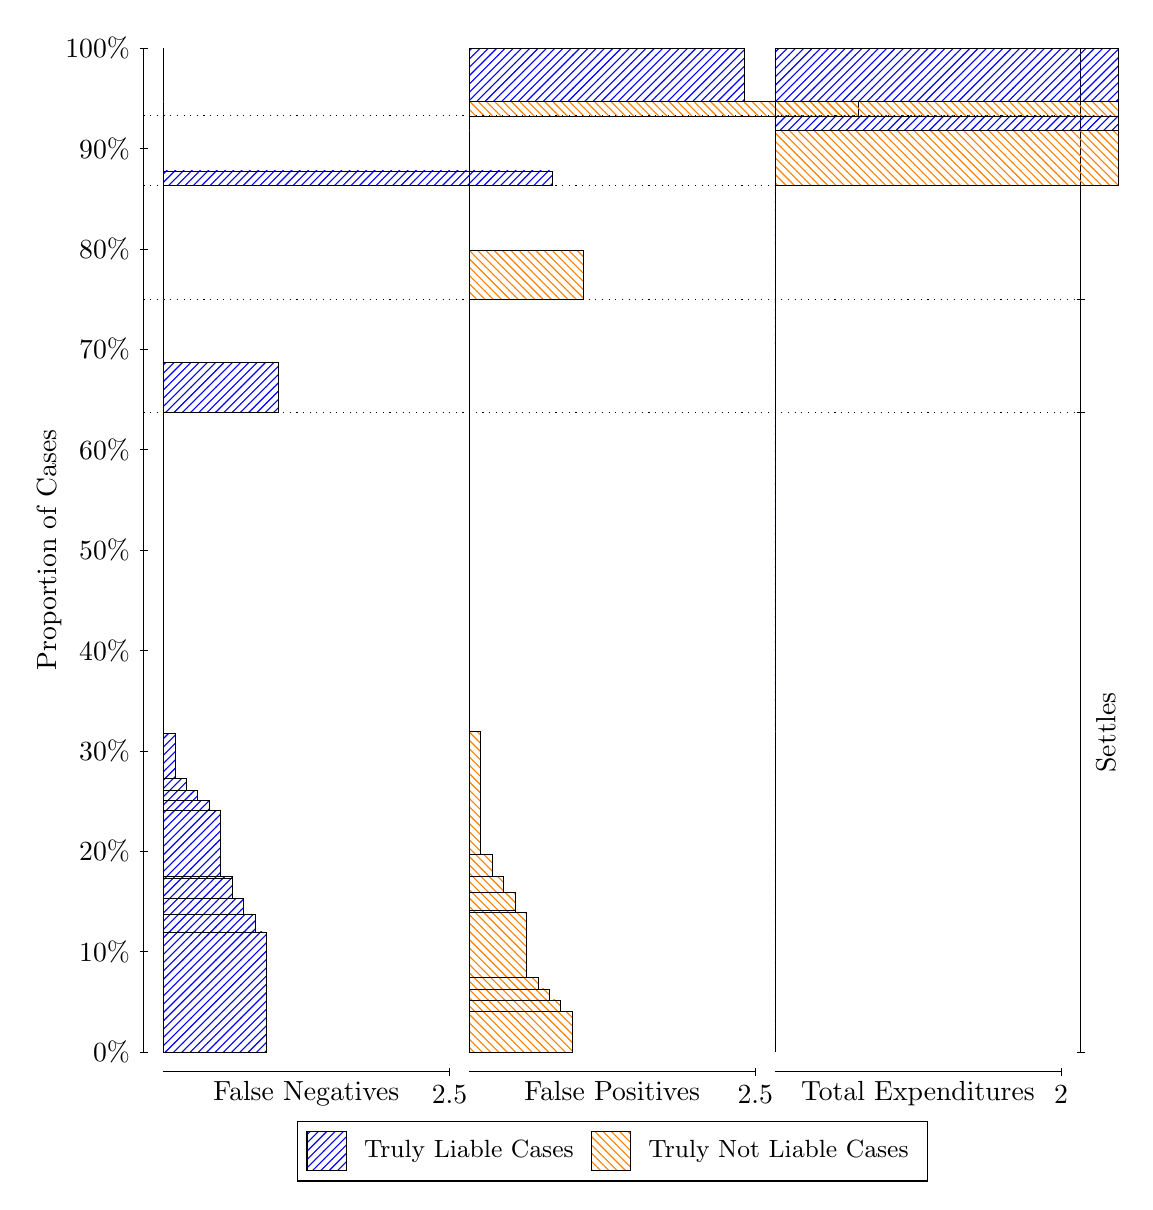
\begin{tikzpicture}
\draw[black, very thin] (1.5,1.75) -- (1.5,14.5);
\node[rotate=90, text=black, anchor=center] at (0.3, 8.125) {Proportion of Cases};
\draw[black, very thin] (1.45,1.75) -- (1.55,1.75);
\node[text=black, anchor=east] at (1.45, 1.75) {0\%};
\draw[black, very thin] (1.45,3.025) -- (1.55,3.025);
\node[text=black, anchor=east] at (1.45, 3.025) {10\%};
\draw[black, very thin] (1.45,4.3) -- (1.55,4.3);
\node[text=black, anchor=east] at (1.45, 4.3) {20\%};
\draw[black, very thin] (1.45,5.575) -- (1.55,5.575);
\node[text=black, anchor=east] at (1.45, 5.575) {30\%};
\draw[black, very thin] (1.45,6.85) -- (1.55,6.85);
\node[text=black, anchor=east] at (1.45, 6.85) {40\%};
\draw[black, very thin] (1.45,8.125) -- (1.55,8.125);
\node[text=black, anchor=east] at (1.45, 8.125) {50\%};
\draw[black, very thin] (1.45,9.4) -- (1.55,9.4);
\node[text=black, anchor=east] at (1.45, 9.4) {60\%};
\draw[black, very thin] (1.45,10.675) -- (1.55,10.675);
\node[text=black, anchor=east] at (1.45, 10.675) {70\%};
\draw[black, very thin] (1.45,11.95) -- (1.55,11.95);
\node[text=black, anchor=east] at (1.45, 11.95) {80\%};
\draw[black, very thin] (1.45,13.225) -- (1.55,13.225);
\node[text=black, anchor=east] at (1.45, 13.225) {90\%};
\draw[black, very thin] (1.45,14.5) -- (1.55,14.5);
\node[text=black, anchor=east] at (1.45, 14.5) {100\%};

\draw[black, very thin] (13.4,1.75) -- (13.4,14.5);
\draw[black, very thin] (13.35,1.75) -- (13.45,1.75);
\node[anchor=west] at (13.35, 1.75) {};
\draw[black, very thin] (13.35,9.8693) -- (13.45,9.8693);
\node[anchor=west] at (13.35, 9.8693) {};
\draw[black, very thin] (13.35,11.305) -- (13.45,11.305);
\node[anchor=west] at (13.35, 11.305) {};
\draw[black, very thin] (13.35,12.755) -- (13.45,12.755);
\node[anchor=west] at (13.35, 12.755) {};
\draw[black, very thin] (13.35,13.639) -- (13.45,13.639);
\node[anchor=west] at (13.35, 13.639) {};
\draw[black, very thin] (13.35,14.5) -- (13.45,14.5);
\node[anchor=west] at (13.35, 14.5) {};

\draw[black, very thin, pattern color=blue, pattern=north east lines] (1.75,1.75) rectangle (3.058,3.274);
\draw[black, very thin, pattern color=blue, pattern=north east lines] (1.75,3.274) rectangle (2.9127,3.5002);
\draw[black, very thin, pattern color=blue, pattern=north east lines] (1.75,3.5002) rectangle (2.7673,3.7042);
\draw[black, very thin, pattern color=blue, pattern=north east lines] (1.75,3.7042) rectangle (2.622,3.9558);
\draw[black, very thin, pattern color=blue, pattern=north east lines] (1.75,3.9558) rectangle (2.622,3.9782);
\draw[black, very thin, pattern color=blue, pattern=north east lines] (1.75,3.9782) rectangle (2.4767,4.8187);
\draw[black, very thin, pattern color=blue, pattern=north east lines] (1.75,4.8187) rectangle (2.3313,4.9443);
\draw[black, very thin, pattern color=blue, pattern=north east lines] (1.75,4.9443) rectangle (2.186,5.0739);
\draw[black, very thin, pattern color=blue, pattern=north east lines] (1.75,5.0739) rectangle (2.0407,5.2291);
\draw[black, very thin, pattern color=blue, pattern=north east lines] (1.75,5.2291) rectangle (1.8953,5.8009);
\draw[black, very thin, pattern color=orange, pattern=north west lines] (1.75,5.8009) rectangle (1.75,9.8693);
\draw[black, very thin, pattern color=blue, pattern=north east lines] (1.75,9.8693) rectangle (3.2033,10.51);
\draw[black, very thin, pattern color=orange, pattern=north west lines] (1.75,10.51) rectangle (1.75,11.305);
\draw[black, very thin, pattern color=orange, pattern=north west lines] (1.75,11.305) rectangle (1.75,11.933);
\draw[black, very thin, pattern color=blue, pattern=north east lines] (1.75,11.933) rectangle (1.75,12.755);
\draw[black, very thin, pattern color=blue, pattern=north east lines] (1.75,12.755) rectangle (6.6913,12.939);
\draw[black, very thin, pattern color=orange, pattern=north west lines] (1.75,12.939) rectangle (1.75,13.639);
\draw[black, very thin, pattern color=orange, pattern=north west lines] (1.75,13.639) rectangle (1.75,13.823);
\draw[black, very thin, pattern color=blue, pattern=north east lines] (1.75,13.823) rectangle (1.75,14.5);
\draw[black, very thin, pattern color=orange, pattern=north west lines] (5.6333,1.75) rectangle (6.9413,2.2702);
\draw[black, very thin, pattern color=orange, pattern=north west lines] (5.6333,2.2702) rectangle (6.796,2.4119);
\draw[black, very thin, pattern color=orange, pattern=north west lines] (5.6333,2.4119) rectangle (6.6507,2.5516);
\draw[black, very thin, pattern color=orange, pattern=north west lines] (5.6333,2.5516) rectangle (6.5053,2.6943);
\draw[black, very thin, pattern color=orange, pattern=north west lines] (5.6333,2.6943) rectangle (6.36,3.5274);
\draw[black, very thin, pattern color=orange, pattern=north west lines] (5.6333,3.5274) rectangle (6.2147,3.5511);
\draw[black, very thin, pattern color=orange, pattern=north west lines] (5.6333,3.5511) rectangle (6.2147,3.7809);
\draw[black, very thin, pattern color=orange, pattern=north west lines] (5.6333,3.7809) rectangle (6.0693,3.9816);
\draw[black, very thin, pattern color=orange, pattern=north west lines] (5.6333,3.9816) rectangle (5.924,4.2615);
\draw[black, very thin, pattern color=orange, pattern=north west lines] (5.6333,4.2615) rectangle (5.7787,5.8184);
\draw[black, very thin, pattern color=blue, pattern=north east lines] (5.6333,5.8184) rectangle (5.6333,9.8693);
\draw[black, very thin, pattern color=orange, pattern=north west lines] (5.6333,9.8693) rectangle (5.6333,10.664);
\draw[black, very thin, pattern color=blue, pattern=north east lines] (5.6333,10.664) rectangle (5.6333,11.305);
\draw[black, very thin, pattern color=orange, pattern=north west lines] (5.6333,11.305) rectangle (7.0867,11.933);
\draw[black, very thin, pattern color=blue, pattern=north east lines] (5.6333,11.933) rectangle (5.6333,12.755);
\draw[black, very thin, pattern color=orange, pattern=north west lines] (5.6333,12.755) rectangle (5.6333,13.455);
\draw[black, very thin, pattern color=blue, pattern=north east lines] (5.6333,13.455) rectangle (5.6333,13.639);
\draw[black, very thin, pattern color=orange, pattern=north west lines] (5.6333,13.639) rectangle (10.575,13.823);
\draw[black, very thin, pattern color=blue, pattern=north east lines] (5.6333,13.823) rectangle (9.1213,14.5);
\draw[black, very thin, pattern color=orange, pattern=north west lines] (9.5167,1.75) rectangle (9.5167,5.8184);
\draw[black, very thin, pattern color=blue, pattern=north east lines] (9.5167,5.8184) rectangle (9.5167,9.8693);
\draw[black, very thin, pattern color=orange, pattern=north west lines] (9.5167,9.8693) rectangle (9.5167,10.664);
\draw[black, very thin, pattern color=blue, pattern=north east lines] (9.5167,10.664) rectangle (9.5167,11.305);
\draw[black, very thin, pattern color=orange, pattern=north west lines] (9.5167,11.305) rectangle (9.5167,11.933);
\draw[black, very thin, pattern color=blue, pattern=north east lines] (9.5167,11.933) rectangle (9.5167,12.755);
\draw[black, very thin, pattern color=orange, pattern=north west lines] (9.5167,12.755) rectangle (13.877,13.455);
\draw[black, very thin, pattern color=blue, pattern=north east lines] (9.5167,13.455) rectangle (13.877,13.639);
\draw[black, very thin, pattern color=orange, pattern=north west lines] (9.5167,13.639) rectangle (13.877,13.823);
\draw[black, very thin, pattern color=blue, pattern=north east lines] (9.5167,13.823) rectangle (13.877,14.5);
\draw[black, dotted] (1.5,9.8693) -- (13.4,9.8693);
\draw[black, dotted] (1.5,11.305) -- (13.4,11.305);
\draw[black, dotted] (1.5,12.755) -- (13.4,12.755);
\draw[black, dotted] (1.5,13.639) -- (13.4,13.639);
\draw[black, very thin] (1.75,1.5) -- (5.3833,1.5);
\node[text=black, anchor=north] at (3.5667, 1.5) {False Negatives};
\draw[black, very thin] (5.3833,1.45) -- (5.3833,1.55);
\node[text=black, anchor=north] at (5.3833, 1.45) {2.5};

\draw[black, very thin] (5.6333,1.5) -- (9.2667,1.5);
\node[text=black, anchor=north] at (7.45, 1.5) {False Positives};
\draw[black, very thin] (9.2667,1.45) -- (9.2667,1.55);
\node[text=black, anchor=north] at (9.2667, 1.45) {2.5};

\draw[black, very thin] (9.5167,1.5) -- (13.15,1.5);
\node[text=black, anchor=north] at (11.333, 1.5) {Total Expenditures};
\draw[black, very thin] (13.15,1.45) -- (13.15,1.55);
\node[text=black, anchor=north] at (13.15, 1.45) {2};

\node[text=black, centered, rotate=90] at (13.72, 5.8096) {Settles};





\draw (7.449999999999999,1.5) node[draw=none] (baseCoordinate) {};
\begin{scope}[align=center]
        \matrix[scale=0.5, draw=black, below=0.5cm of baseCoordinate, nodes={draw}, column sep=0.1cm]{
            \node[rectangle, draw, minimum width=0.5cm, minimum height=0.5cm, pattern color=blue, pattern=north east lines] {}; &
            \node[draw=none, font=\small, text=black] (B) {Truly Liable Cases}; &
            \node[rectangle, draw, minimum width=0.5cm, minimum height=0.5cm, pattern color=orange, pattern=north west lines] {}; &
            \node[draw=none, font=\small, text=black] (B) {Truly Not Liable Cases}; \\
            };
\end{scope}

\end{tikzpicture}
\end{document}